\documentclass{article}
\usepackage{algorithmicx}
\usepackage{algpseudocode}
\usepackage{graphicx}
\usepackage{color}
\usepackage[utf8]{inputenc}
\begin{document}
{\noindent \Huge Problema a resolver:}
\newline \newline  El problema esta dado por la siguiente situaci\'on: 
tenemos en un $"$lista$"$ con una cantidad \textit{3$*$n} de n\'umeros(n un n\'umero fijo).\newline
Para \textit{i} desde \textit{0} a \textit{n-1}, vamos a decir que la posici\'on \textit{i} en la lista va a ser \textit{Izq} del edificio \textit{i-\'esimo}, \textit{i+1} va a ser \textit{Alt} del edificio \textit{i-\'esimo} e \textit{i+2} va a ser \textit{Der} del edificio i-\'esimo.\newline
A grandes rasgos vamos a tener una lista de \textit{n} edificios (interpretamos a un edificio como una tupla \textit{$<$Izq,Alt,Der$>$}) con una base en com\'un impl\'icita que es 0.\newline
Vamos a utilizar esta notación para referirnos a los edificios.\newline
Por ejemplo para un entrada de la forma: \newline
\textit{lista={1,2,3,4,2,7,2,4,6}} y 
\textit{n=3} tendr\'iamos: \newline 
\textit{lista$=$ $<$1,2,3$>$,$<$4,2,7$>$,$<$2,4,6$>$}\newline 
Proyectada en un gr\'afico quedar\'ia: \newline
\vspace{0.4cm}
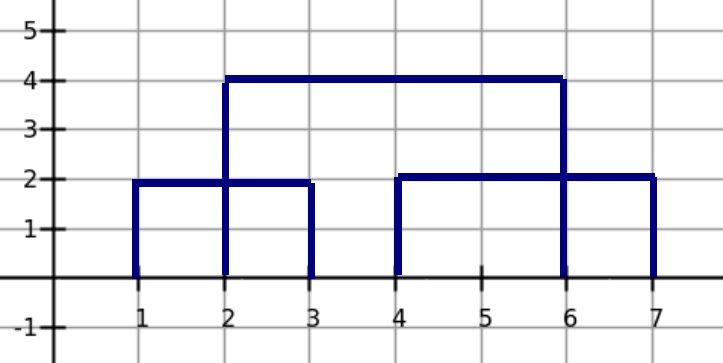
\includegraphics[width=\textwidth,height=\textheight,keepaspectratio
]{edificiosGraf1.png}
\begin {flushleft}
\end{flushleft}
Lo que queremos hacer es $"$eliminar todas las lineas interiores del gr\'afico$"$, quedarnos con su contorno (se obtiene el mismo resultado  "siguiendo con el dedo el gr\'afico") para luego poder dar la solución final que explicaremos más adelante. \newpage
Veamos un ejemplo de eliminación de lineas interiores y el "procedimiento" de seguir con el dedo el gráfico \newline
Para una \textit{lista$=$ $<$0,3,8$>$,$<$1,6,5$>$,$<$2,4,6$>$,$<$4,2,7$>$,$<$9,6,10$>$} con \textit{n=5},\newline su gr\'afico es: \newline
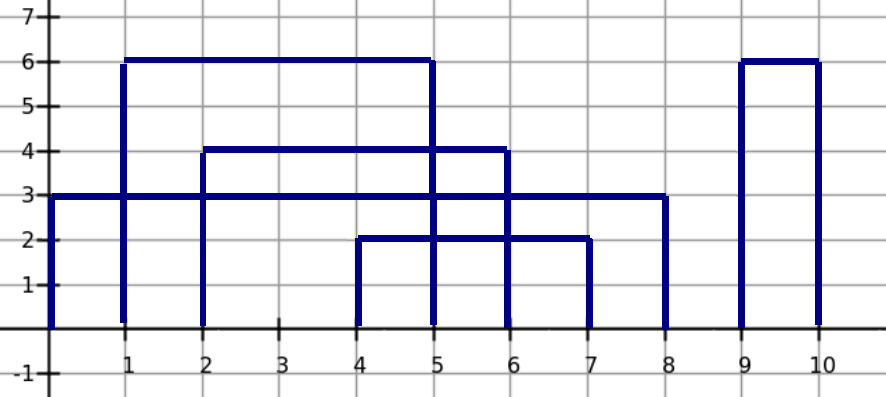
\includegraphics[width=\textwidth,height=\textheight,keepaspectratio
]{edificiosGraf2.png}
\begin {flushleft}
\end{flushleft}
el gr\'afico de eliminar las lineas interiores es:\newline
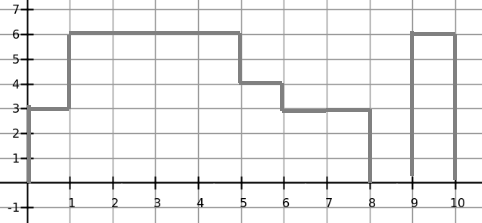
\includegraphics[width=\textwidth,height=\textheight,keepaspectratio
]{edificiosGraf2b.png}
\begin {flushleft}
\end{flushleft}
\newpage
Mientras que el gr\'afico de "seguir con el dedo" es: \newline
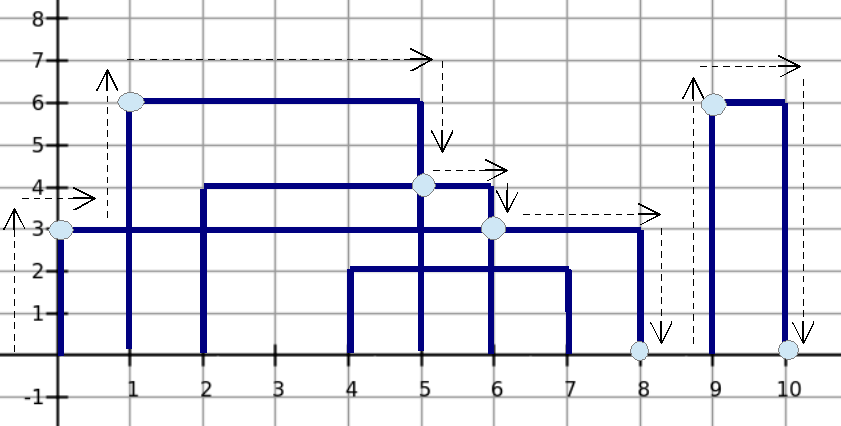
\includegraphics[width=\textwidth,height=\textheight,keepaspectratio
]{edificiosGraf2c.png}
\begin {flushleft}
La salida para este ejemplo sería:\newline \textit{{0,3,1,6,5,4,6,3,8,0,9,6,0}}
\end{flushleft}
Lo que hago cuando "sigo con el dedo" es: \newline
Empezar con el primer edificio y seguir el trazo, si me interseco con otro edificio seguir el trazo del edificio con el que me intersequ\'e desde ese punto. \newline
Si no me interseco con nadie, pero hay m\'as edificios adelante "seguir con el dedo" los otros. Si no hay más edificios termin\'e.\newline
Luego de ese contorno voy a obtener la soluci\'on final que son los puntos donde hay cambios de altura($\uparrow$ $\longrightarrow$ y $\downarrow$ $\longrightarrow$). \newline
\newpage
{\noindent \Huge Resoluci\'on:}
\newline \newline
Un panorama de la resolución es:\newline
ordenar los edificios de menor a mayor por su \textit{Izq} (en caso que tengan mismo \textit{Izq} es menor el que tiene mayor \textit{Alt}). \newline
Agregar a la solución el primer punto del primer edifico de la lista de edificios ordenada. \newline
Vamos a ir recorriendo los edificios, voy a tener un edificio \textit{comparo} en este recorrido(al principio \textit{comparo} es el primer edificio) y empiezo a recorrer desde el segundo, en caso de haber más de uno,el edificio por el que voy será \textit{siguiente}. También tengo una \textit{cola} de prioridad (organizada por mayor Alt) donde voy a ir metiendo edificios.\newline
Si \textit{comparo} interseca a \textit{siguiente}:\newline
agrego a la solución el cambio de altura si \textit{siguiente.Alt} $>$ \textit{comparo.Alt}.\newline
Si \textit{siguiente.Altura $>=$ comparo.Alt} , ahora \textit{comparo} es \textit{siguiente} y encolo a \textit{comparo} en la \textit{cola}.\newline
Si \textit{siguiente.Alt $<$ comparo.Alt} encolo a siguiente en la \textit{cola} y \textit{comparo} queda donde estaba.\newline
 
Si \textit{comparo} no interseca a \textit{siguiente}\newline
Quiere decir que están "separados",pero puede que haya un edificio $e$ tal que \textit{e.Izq $<=$ comparo.Izq}, \textit{e.Der $>$ comparo.Der} y \textit{e.Alt $<=$ comparo.Alt}, si existiera $e$ tendría que estar en la cola.)\newline
Si la \textit{cola} no está vacía voy a buscar a $e$ en la \textit{cola}(si existe, lo encolé cuando fui viendo los edificios anteriores a \textit{siguiente}):\newline
si el tope de la \textit{cola} es $e$, ahora $e$ es comparo, agrego a la solución la intersección por derecha de $e$ con $comparo$, no lo desencolo porque pude que corte a otros edificios de más adelante.\newline
Si el tope de la $cola$ no es $e$ desencolo y sigo buscando.
Si la \textit{cola} es vacía(quiere decir que no había ningún edificio que terminara \newline después que comparo) agrego a la solución el final de \textit{comparo} y el principio de \textit{siguiente}, ahora \textit{comparo} es \textit{siguiente}.
\newline
Terminé de recorrer los edificios,pero puede que hayan quedado cosas dentro de la \textit{cola} y parte de la solución no la esté dando.\newline
Mientras la \textit{cola} tenga edificios, voy a comparar el tope con \textit{comparo}:\newline
si \textit{tope.Der $<$ comparo.Der} desencolo.\newline
En caso contrario, ahora \textit{comparo} es \textit{siguiente} ,agrego a la solución la intersección por derecha entre el tope y \textit{comparo}, desencolo.\newline
Ya no hay más edificios en la \textit{cola}.
Agregar a la solución el último punto \textit{comparo.Der},\textit{0} y retornar la solución.
\newline
Hay cosas que en esta descripción no tuve en cuenta, porque son muy especificas, para explicarlo profundamente lo hago con este pseudocódigo: 
\newpage
 
Sea lista: lista(\textit{números}) de longitud \textit{3*n} y \textit{n} la cantidad de edificios
\vspace{0.4cm}
\begin{algorithmic}[1]
\Procedure{ResolverEdificios}{$lista$,$n$}
        \State $\textit{pasar a tuplas ($<$Izq,Alt,Der$>$) la lista}$
        \State $\textit{ordenar los edificios por Izq, en caso de tener mismo Izq es menor el que tiene mayor Alt}$
        \State $comparo\gets lista[0]$
        \State $cola\gets \textit{vacía}$
        \State $\textit{imprimo el primer punto(comparo.Izq y comparo.Alt)}$
        \For{$(i\gets 1, n-1)$} \textit{$//$voy recorriendo los edificios a partir del segundo}
                \State $siguiente\gets lista[i]$
                \If{$(\textit{comparo.Der $>=$ iguiente.Izq(se intersecan)})$}
                        \If{$(\textit{siguiente.Alt $>$ comparo.Alt})$}
                                \State $\textit{imprimir cambio de altura(\textit{siguiente.Der, siguiente.Alt})}$
                                \State$\textit{si la cola está vacia encolar comparo, sino, encolar comparo si el tope no es comparo}$                          
                                        \State $comparo\gets siguiente$
                        \EndIf
                        \If{$(\textit{siguiente.Alt $==$ comparo.Alt})$}
                                \State$\textit{si la cola está vacia encolar comparo, sino, encolar comparo si el tope no es comparo}$                          
                        \EndIf
                        \If{$(\textit{siguiente.Alt $<$ comparo.Alt})$}
                                \State $\textit{encolar comparo}$
                        \EndIf
                        
                \Else \textit{(no se intersecan comparo y siguiente)}
                        \If{$(\textit{la cola no está vacía})$}                                                                         
                                \While{$(\textit{cola no vacía})$}
                                        \If{$(\textit{topeCola.Der $<$ comparo.Der})$}          
                                        \State $\textit{desencolar}$
                                        \Else 
                                        \State $\textit{imprimir intersección entre comparo y topeCola(comparo.Der,topeCola.Alt)}$
                                        \State $comparo\gets topeCola$
                                        \State $\textit{salir del while}$
                                        \EndIf
                                \EndWhile
                        \Else{\textit{ //no pasé a nadie que cortaría a comparo, como no se intersecan comparo y siguiente imprimo ambos puntos}}
                        \State $\textit{imprimir comparo.Der, 0 }$
                        \State $\textit{imprimir siguiente.Izq, siguiente.Alt}$
                        \State $comparo\gets siguiente$
                        \EndIf
                \EndIf
        \EndFor\textit{//terminé de iterar los edificios,puede que hayan quedado cosas en el cola,uso a comparo que es el último edificio visto con el que haya en el tope de la cola} \newpage
        
        \For{$(\textit{la cola no es vacía}, \textit{desencolar})$}
                \If{$(\textit{comparo.Der $<=$ topeCola.Der)}$}
                \State $\textit{imprimir intersección por entre comparo y topeCola(comaro.Der,topeCola.Alt)}$
                \EndIf
                \State $\textit{desencolar}$    
        \EndFor
        \State $\textit{al último punto no lo imprimo nunca)}$
        \State $\textit{$//$lo imprimo acá}$
        \State $\textit{imprimir comparo.Der y 0}$
\EndProcedure
\end{algorithmic}
\newpage
{\noindent \Huge Complejidad:}
\newline \newline
Al principio del algoritmo paso la lista de edificios a una lista de tuplas:
cada \textit{3} números voy a formar una tupla(la cantidad de números totales es \textit{3*n}), el costo de crear una tupla es \textit{c}(de asignaciones y crear cosas que son 1 operación) y de ubicarla en una lista es también 1 operación.\newline
Entonces recorro \textit{3*n} números y cada \textit{3} creo un edificio, con lo cuál hago \textit{3*n*(c+1)} para convertir a tuplas los edificios.\newline
Luego de convertirlos a tuplas,ordeno los edificios por Izq(en caso de igual Izq es menor el de mayor Alt), el costo de ordenarlos es \textit{n*log(n)} (porque uso sort de la stl \textit{http://www.cplusplus.com/reference/algorithm/sort/?kw=sort} ).\newline
Vamos a ver que la cantidad de veces que encolo es una función de n, y así poder ver que la cantidad de veces que desencolo es también una función de n porque no puedo desencolar más cosas de las que encolo.
Vemos en el algoritmo que en  \textit{*1} y \textit{*2}, encola si está vacía o si el tope de la cola no es comparo. Luego en \textit{*3} encolo. Después a lo largo de todo el algoritmo no hago \textit{nunca} un encolar.\newline
Como todos estos casos son disjuntos (o son $<$,$>$ o $=$ Alt de \textit{comparo} y \textit{siguiente}) entonces hago 1 encolar en cada edificio en peor caso, con lo cual hago \textit{n} encolar. 
\newline
Veamos ahora la cantidad de operaciones del \textit{while} dentro del \textit{for}(de recorrer los edificios), en peor caso por cada edificio desencolo todos los edificios, eso da una complejidad \textit{n*(n*(costo de desencolar))}. Pero si analizamos más finamente, nunca podría para cada paso desencolar todos los edificios.\newline
Recorriendo los edificios ordenados(\textit{línea 3 pseudo}), si voy por el edificio \textit{i} (\textit{i} entre \textit{0} y \textit{n-1}), tengo en la cola en peor caso \textit{i} edificios(por lo explicado arriba de la cantidad de encolar), entro en el \textit{while}(suponiendo que los edificios \textit{i} e \textit{i+1(en caso de existir)} no se tocan) y desencolo \textit{i} edificios(en peor caso desencolo todos los que encolé), sigo avanzando y llego a un edificio \textit{j} (\textit{j} entre \textit{i} y \textit{n-1} ) ahora en la cola en peor caso tengo \textit{j-i} edificios(pues los edificios anteriores a \textit{i} ya no están en la cola y encolé todos desde \textit{i} hasta \textit{j}), entro en el \textit{while}(suponiendo que los edificios j y j+1(en caso de existir) no se tocan) y desencolo en peor caso \textit{j-i} edificios.
Llego al último edificio \textit{n-1} y en peor caso tengo \textit{n-1-j} edificios en en la cola(porque los edificios hasta \textit{j} no están en la cola porque los desencolé), entro al \textit{while} y desencolo \textit{n-1-j} veces.\newline
Si sumo la cantidad de veces que hice desencolar en el recorrido de los edificios es \textit{n} (suma de los intervalos).
Entonces hago \textit{n} veces desencolar en peor caso 
Relacionando la parte de encolar y desencolar en el primer \textit{for}
por cada edificio hago un encolar y una cantidad \textit{x} de desencolar + c(\textit{constante}) operaciones que tienen costo 1 (asignaciones y guardas).\newline
Por lo visto anteriormente la suma de esos \textit{x} es \textit{n}, entonces el costo del \textit{while} dentro de primer \textit{for} es  \textit{n*(costo de encolar)+ n*(costo de desencolar) +n*c(constante)} operaciones
\newline
Para  el segundo \textit{for}, en peor caso tengo todos los edificios que son \textit{n} en la cola, y desencolo hasta que se vacia,entonces hace \textit{n*(costo de desencolar) + c1}(constante de guardas y asignaciones)) operaciones\newline
En la implementación usamos una priority-queue como cola, el costo de encolar(push) es log(n),desencolar(pop) es log(n) y tope(top) es 1. \textit{http://www.cplusplus.com/search.do?q=priority}
\newline
Finalmente la complejidad es \newline
O(\textit{3*n*(c+1) de crear las tuplas}\newline
+\textit{n*log(n) de ordenarlos} \newline
+ \textit{n*c+n[\textit{encolar}]+n*(log(n))[\textit{desencolar}] del primer for} \newline
+ \textit{n*c + n*log(n)[\textit{desencolar}] del segundo for})  = \newline
\textit{0((3*(c+1)+c+1+c)*n + 3*n*(log(n))} \newline
$\in$ O(n(log(n))) (acoto por el máximo y saco las constantes)\newline
\newpage
{\noindent \Huge Correctitud:}
\newline \newline
El algoritmo pone en la solución (\textit{primerEdificio.Izq,primerEdificio.Alt}).\newline
En la solución al problema, el primer "punto" es \textit{Der, Alt del edificio} que tiene menor \textit{Izq} y mayor \textit{Alt} que todos, ya que es el primer cambio de altura.
¿El primer punto que pone mi algoritmo cumple con dichas propiedades?
Veamos, paso los numeros de la entrada a tuplas, ordeno los edificios(en tuplas) por \textit{Izq} (linea 3).
Entonces el primer edificio va a ser el de menor \textit{Izq} y el de mayor \textit{Alt}.\newline
Con lo cual si, el primer punto cumple con esas propiedades.
\newline
Voy iterando los edificios mirando el edificio por el que voy(\textit{siguiente}) y un edificio que voy marcando en ciertos casos, \textit{comparo}. \textit{Comparo} no necesariamente es uno menos que \textit{siguiente}.
Al principio del algoritmo \textit{comparo} es el primer edificio y \textit{siguiente} el segundo en caso de haber.\newline
Si \textit{comparo.Der} $>=$ \textit{siguiente.Izq} (se intersecan):\newline
si \textit{comparo.Alt} $<$ siguiente.Alt \newline
                tengo que poner el punto de cambio de altura, $p$, en la solución\newline
                Supongamos no tengo que poner a $p$ en la solución:\newline
                        caso existe un edificio, $e$ que cumple: \textit{e.Izq $<$ siguiente.Izq}, \textit{e.Alt $>$ siguiente.Alt} y \textit{e.Der $>=$ siguiente.Der}(este edificio tapa al punto que quiero agregar a la solución):\newline
\color{red}{(ejemplo grafico C)} \color{black} \newline
                        Si existiera tendría que haberlo puesto como comparo,pero estoy en el caso donde la altura de comparo es menor que la de siguiente, el edificio no puede existir. Entonces hay que poner a $p$ en la solución.\newline
Si no se intersecan \textit{comparo} y \textit{siguiente}:\newline
\color{red}{(grafico no se intersecan)} \color{black} \newline
        voy a tener en la cola los edificios que tienen \textit{Der} mayor a \textit{comparo.Der} porque los fui enconlando, en caso de existir, entre otros.\newline
        si la cola está vacía quiere decir que no hay nadie que corte a \textit{comparo}(Gráfico cola vacia grafico),entonces el edificio \textit{comparo} sigue hasta su base y tengo que seguir con los demás edificios(en caso de tener más) desde \textit{siguiente}, entonces voy a poner en la solución, el final de comparo (comparo.Der, 0) y el principio de siguiente(siguiente.Izq, siguiente.Alt).\newline

        Si la cola no está vacía quiere decir que puede que tenga un edificio que corte a \textit{comparo} por \textit{Der}.
\color{red}{Grafico que corte a comparo}\color{black} \newline
                Voy a buscar un edificio que interseque a \textit{comparo} por \textit{Der}(si lo encuentro no busco más),mirando el tope, en este caso no voy a desencolar. Si el tope no es lo que busco desencolo. \newline
                Por como es la cola este que quería encontrar es el que tiene mayor \textit{Alt} de los edificios que tienen menor \textit{Alt} que \textit{comparo}.
                Entonces este punto,$p$, de intersección lo agrego a la solución.\newline
                Supongamos que no tengo que agregar a $p$ a la solución.\newline
                caso existe un edificio,$e$, que cumple que: \textit{e.Izq $<$ comparo.Izq}, \textit{e.Der $>$ comparo.Der} y \newline
                \textit{comparo.Alt $<=$ e.Alt $<$ topeCola.Alt} \newline
\color{red}{(grafico E)} \color{black} \newline          
                 Entonces este si existiera, lo tendría que haber encolado cuando recorría los edificios y tendría que ser el edificio que me daría el tope de la cola Absurdo!. Entonces tengo que agregar a $p$ a la solución.\newline
Siempre recorro los edificios mirando \textit{comparo} y \textit{siguiente}, en algún momento me voy a quedar sin edificios, \textit{comparo} va a quedar en algún edificio y la cola va a tener algún estado (vacía o con edificios dentro) \newline
\color{red}{ejemplos de estados de la cola}\color{black}\newline
Ahora voy a trabajar con \textit{comparo} y la \textit{cola} (ahora en la cola están mis "siguientes")
Si hay edificios en la cola:
Quiere decir que uno de esos edificios interseque en Der a comparo.\newline
Hasta que esté vacía la cola voy a buscar el edificio que interseque a \textit{comparo} por \textit{Der},mirando el tope, si no está el tope desencolo. Si lo encuentro ahora ese es comparo y desencolo. \newline
                Por como es la cola este que quería encontrar es el que tiene mayor \textit{Alt} de los edificios que tienen menor \textit{Alt} que \textit{comparo}.
                Entonces este punto,$p$, de intersección lo agrego a la solución.\newline
                Supongamos que no tengo que agregar a $p$ a la solución.\newline
                caso existe un edificio,$e$, que cumple que: \textit{e.Izq $<$ comparo.Izq}, \textit{e.Der $>$ comparo.Der} y \newline
                \textit{comparo.Alt $<=$ e.Alt $<$ topeCola.Alt} \newline
\color{red}{(grafico E)} \color{black} \newline          
                 Entonces este si existiera, lo tendría que haber encolado cuando recorría los edificios y tendría que ser el edificio que me daría el tope de la cola Absurdo!. Entonces tengo que agregar a $p$ a la solución.\newline

A lo sumo voy a poner un punto en cada iteración, si pongo ese punto, entonces va a ser entre \textit{comparo} y el edificio \textit{E} de mayor Alt que lo pase por Der. Supongo que ese punto de intersección no es valido, entonces existe otro edificio \textit{E'} de mayor Alt que \textit{E} y que termine después que \textit{comparo} (\textit{E'} tapa al punto de intersección)
\newline
Si  \textit{E'.Alt $>$ comparo.Alt}, entonces llegamos a un absurdo ya que \textit{E'} debería ser \textit{comparo} porque solo cambio a \textit{comparo} cuando el que saque de la cola lo pasa por \textit{Der} y tiene mayor Alt, Absurdo!. 
Si la altura de \textit{E'.Alt} $<=$ comparo.Alt, entonces como la altura de \textit{E'} es mayor que la de \textit{E} (para que tape el punto de intersección), tendría que ser  \textit{E'} el tope de la cola y no \textit{E}, Absurdo.Con lo cual el punto es valido.\newline
Demostramos que todos los puntos que pone nuestro algoritmo son válidos.\newline
Ahora tenemos que demostrar que esos puntos son todos los de la solución, osea que no olvidamos ninguno.
Sea \textit{S} la solución (de puntos ordenados) al problema, quiero ver que todos los puntos de \textit{S} están en la solución que dí. 
El primer punto sabemos que lo vamos a poner siempre porque está al principio del algoritmo
El resto de los puntos exceptuando el primero, podemos dividirlos en \textit{ascendentes} (cuando el punto anterior es mas bajo), \textit{descendentes} (cuando el punto anterior es mas alto) y cambios de altura a 0.
Dado cualquier punto descendente de \textit{S} con altura distinta de 0, quiero ver que está en la solución que devuelve el algoritmo. Como la altura es distinta de cero, entonces el punto debe ser la intersección entre dos edificios \textit{E1} (mayor altura) y \textit{E2} (menor altura). Si podemos probar que eventualmente va a valer \textit{comparo = E1}, entonces estaríamos probando que vamos a poner el punto en la solución ya que vimos que, como en la cola tenemos todos los edificios menores que \textit{comparo} que terminan despues que \textit{comparo} (entre otros más que también pueden estar en la cola), vamos a desencolarlo y agregar el punto a la solución. \newline
Supongamos que no existe ningun estado del algoritmo en el cual \textit{comparo = E1}, entonces seguro existe un edificio \textit{E'} tal que tapa a \textit{E1} ya que, nuestro algoritmo cambia el valor de \textit{comparo} cuando encuentra un \textit{siguiente} tal que la altura de \textit{siguiente} es mayor a la de \textit{comparo} o, cuando estoy desencolando pero cuando desencolo me quedo con los que terminan despues de \textit{comparo} y, si \textit{E'} tapa totalmente a \textit{E1} entonces \textit{E1} va a ser desencolado pero no va a terminar después que \textit{comparo} y por lo tanto comparo no va a cambiar de valor. Pero, si existe \textit{E'} tal que tapa a \textit{E1}, entonces particularmente va a tapar al punto de interseccion denotado por \textit{E1} y \textit{E2}, entonces ese punto no va a ser solucion y habiamos supuesto que si lo era. Llegamos a un absurdo proveniente de suponer que existe una solucion denotada por dos edificios \textit{E1} y \textit{E2} y que \textit{E1} es distinto a \textit{comparo} para cualquier estado del algoritmo. Por lo tanto, \textit{E1 = comparo} para algun estado del algoritmo y entonces eventualmente vamos a llegar a identificar el punto de intersección cuando desencolemos.


Ahora, queremos ver que vamos a agregar todos los cambios de altura a cero.
Dado que en cada iteración me fijo si el \textit{siguiente} edificio interseca a \textit{comparo} y, en el caso de que no lo interseque y la cola vacía entonces agrego el punto, si pasa esto quiere decir que no existe ningún edifició que termine después de \textit{comparo} y empiece antes de que finalice \textit{comparo}. Por lo tanto \textit{comparo} es el último edificio antes del espacio denotado por el cambio de altura a 0. Entonces el punto es efectivamente una solución. \newline
Si la cola tiene edificios, quiere decir que pueden existir edificios que terminan después que \textit{comparo} y, como voy a actualizar el valor de \textit{comparo} al edificio más alto de la cola que termine despues que el edificio que contiene "ahora" \textit{comparo}, si efectivamente existía un espacio entre dos edificios (un cambio de altura a 0), entonces lo voy a detectar. ya que voy a repetir este procedimiento por cada edificio que no esté contenido por otro (porque va a ser comparo).
Luego para los puntos ascendentes:
Como por cada iteración nos fijamos si la altura de \textit{comparo} es menor a la altura de \textit{siguiente} y, en el caso de que se intersequen, agregamos el punto (\textit{siguiente.Izq, siguiente.Alt}) a la solución.\newline
 Además, en el caso de que haya un cambió de altura a 0 y existe un edificio \textit{siguiente}, ya demostramos que ese cambio de altura lo agregamos. Además de agregar ese cambio de altura a 0, agregamos el cambio de altura a la altura de \textit{siguiente}, que representa un punto de altura creciente. Ya que vimos que los cambios de altura a 0 los agregamos todos y que el algoritmo verifica siempre si \textit{comparo} tiene altura menor que un edificio \textit{siguiente} que lo interseca, vemos que no puede existir un punto de crecimiento que no lo agreguemos porque estamos viendo los dos casos donde aparece dicho punto.
 
Con lo dicho anteriormente ya quededa demostrado que todos los puntos de la solución los da el algoritmo.




\newpage
{\noindent \Huge Experimentaci\'on:}
\newline \newline Se han generado 200 instancias donde la instancia $n_i = n_{i-1} + 1000$ y $n_1 = 1000$. Por cada instancia, vale que para todo edificio $e$ generado, $e.Izq < e.Der$ y, tanto $e.Izq$ como $e.Der$ y $e.Alt$ se han elegido de manera aleatoria en el rango [0, 49]. El rango puede sonar arbitrario y, si bien lo es porque podr\'iamos haber elegido otro, tambi\'en resulta razonable desde el punto de vista que permite que, cuando $n$ es muy grande, entonces los edificios se superpongan m\'as, generandose as\'i m\'as intersecciones entre ellos y haciendo que el algoritmo deba trabajar m\'as para decidir cual intersecci\'on es un punto de la soluci\'on y cual no lo es.
\newline Se ha corrido el algoritmo 10 veces sobre cada una de las instancias. Luego, se calcul\'o el tiempo m\'inimo, m\'aximo y promedio por cada instancia, a continuaci\'on mostramos los gr\'aficos correspondientes:

\vspace{2cm}
\includegraphics[width=\textwidth,height=\textheight,keepaspectratio
]{editiempominimo.jpg}
\includegraphics[width=\textwidth,height=\textheight,keepaspectratio
]{editiempomaximo.jpg}

\includegraphics[width=\textwidth,height=\textheight,keepaspectratio
]{editiempopromedio.jpg}

\vspace{2cm}
Dado que nuestro algoritmo va a correr paralelamente con otros procesos, en algunas ejecuciones se va a demorar m\'as que en otras. Tomando el tiempo m\'inimo como el m\'as significativo (es decir, como la ejecuci\'on en la cual fue "menos interrumpido"), si dividimos ese tiempo por $n$, obtenemos el siguiente gr\'afico:

\includegraphics[width=\textwidth,height=\textheight,keepaspectratio
]{editiempolog.jpg}

Con los gr\'aficos anteriores no pod\'iamos decir mucho ya que, aparentemente aproximan a una recta, pero como al dividirlos por $n$ obtenemos una funci\'on que creciente y no una constante, efectivamente ten\'iamos (en el gr\'afico de tiempo m\'inimo) una funci\'on perteneciente a $\Omega(n)$.
\newline Si nuevamente dividimos esta \'ultima funci\'on, esta vez por $log(n)$, obtenemos lo siguiente:

\includegraphics[width=\textwidth,height=\textheight,keepaspectratio
]{editiempoconst.jpg}

Vemos que los puntos parecieran tender al valor 0.003. Si recapitulamos, lo que hicimos fue tomar los valores de tiempo m\'inimo, dividirlos por $n$ y a ese valor dividirlo por $log(n)$ y llegamos a valores que tienden a un n\'umero constante $k \simeq 0.003$.
\newline Si aumentamos a\'un m\'as el $n$ m\'aximo y hacemos este mismo an\'alisis, para instancias de hasta $n = 991000$ obtenemos el siguiente gr\'afico:

\includegraphics[width=\textwidth,height=\textheight,keepaspectratio
]{constanteparangrande.jpg}

en el cual podemos observar que el gr\'afico sigue tendiendo a una constante $\simeq 0.003$.
\newline Concluimos entonces que los tiempos tomados concuerdan con la complejidad te\'orica calculada $O(n.log(n))$
\end{document}
